\documentclass[11pt,addpoints,answers]{exam}

%-----------------------------------------------------------------------------
% PACKAGES AND OTHER DOCUMENT CONFIGURATIONS
%-----------------------------------------------------------------------------

\usepackage[margin=1in]{geometry}
\usepackage{amsmath, amsfonts}
\usepackage{enumerate}
\usepackage{graphicx}
\usepackage{titling}
\usepackage{url}
\usepackage{xfrac}
\usepackage{natbib}
\usepackage{amssymb}
\usepackage{amsthm}
\usepackage{paralist}
\usepackage{epstopdf}
\usepackage{tabularx}
\usepackage{longtable}
\usepackage{multirow}
\usepackage{multicol}
\usepackage[colorlinks=true,urlcolor=blue]{hyperref}
\usepackage{algorithm}
\usepackage{algorithmicx}
\usepackage[noend]{algpseudocode}
\usepackage{float}
\usepackage{enumerate}
\usepackage{array}
\usepackage{environ}
\usepackage{times}
\usepackage{textcomp}
\usepackage{caption}
\usepackage{parskip} % For NIPS style paragraphs.
\usepackage[compact]{titlesec} % Less whitespace around titles
\usepackage[inline]{enumitem} % For inline enumerate* and itemize*
\usepackage{datetime}
\usepackage{comment}
% \usepackage{minted}
\usepackage{lastpage}
\usepackage{color}
\usepackage{xcolor}
\usepackage[final]{listings}
\usepackage{tikz}
\usetikzlibrary{shapes,decorations,quotes, babel}
\usepackage{framed}
\usepackage{booktabs}
\usepackage{cprotect}
\usepackage{verbatim}
\usepackage{verbatimbox}
\usepackage{multicol}
\usepackage{hyperref}
\usepackage{subcaption}
\usepackage{mathtools} % For drcases
\usepackage{cancel}
\usepackage[many]{tcolorbox}
\usepackage{soul}
\usepackage[bottom]{footmisc}
\usepackage{bm}
\usepackage{wasysym}
\usepackage[utf8]{inputenc}
\usepackage{tikz}
\usetikzlibrary{arrows}
\usetikzlibrary{arrows.meta}
\usetikzlibrary{shapes.geometric}
\usetikzlibrary{positioning, arrows, automata, calc}
\usepackage{transparent}

\newtcolorbox[]{your_solution}[1][]{
    % breakable,
    enhanced,
    nobeforeafter,
    colback=white,
    title=Your Answer,
    sidebyside align=top,
    box align=top,
    #1
}

%%%%%%%%%%%%%%%%%%%%%%%%%%%%%%%%%%%%%%%%%%%
% Formatting for \CorrectChoice of "exam" %
%%%%%%%%%%%%%%%%%%%%%%%%%%%%%%%%%%%%%%%%%%%

\CorrectChoiceEmphasis{}
\checkedchar{\blackcircle}

%%%%%%%%%%%%%%%%%%%%%%%%%%%%%%%%%%%%%%%%%%%
% Rotated Column Headers                  %
%%%%%%%%%%%%%%%%%%%%%%%%%%%%%%%%%%%%%%%%%%%
\usepackage{adjustbox}
\usepackage{array}

%https://tex.stackexchange.com/questions/32683/rotated-column-titles-in-tabular

\newcolumntype{R}[2]{%
    >{\adjustbox{angle=#1,lap=\width-(#2)}\bgroup}%
    l%
    <{\egroup}%
}
\newcommand*\rot{\multicolumn{1}{R{45}{1em}}}% no optional argument here, please!

%%%%%%%%%%%%%%%%%%%%%%%%%%%%%%%%%%%%%%%%%%
% Custom commands                        %
%%%%%%%%%%%%%%%%%%%%%%%%%%%%%%%%%%%%%%%%%%

\newcommand{\vc}[1]{\boldsymbol{#1}}
\newcommand{\adj}[1]{\frac{d J}{d #1}}
\newcommand{\chain}[2]{\adj{#2} = \adj{#1}\frac{d #1}{d #2}}

\newcommand{\R}{\mathbb{R}}
\newcommand{\blackcircle}{\tikz\draw[black,fill=black] (0,0) circle (1ex);}
\renewcommand{\circle}{\tikz\draw[black] (0,0) circle (1ex);}

\newcommand{\emptysquare}{{\LARGE $\square$}\ \ }
\newcommand{\filledsquare}{{\LARGE $\blacksquare$}\ \ }
\newcommand{\emptycircle}{{\LARGE $\fullmoon$}\ \ }
\newcommand{\filledcircle}{{\LARGE $\newmoon$}\ \ }

\newcommand{\ntset}{test}

% mathcal
\newcommand{\Ac}{\mathcal{A}}
\newcommand{\Bc}{\mathcal{B}}
\newcommand{\Cc}{\mathcal{C}}
\newcommand{\Dc}{\mathcal{D}}
\newcommand{\Ec}{\mathcal{E}}
\newcommand{\Fc}{\mathcal{F}}
\newcommand{\Gc}{\mathcal{G}}
\newcommand{\Hc}{\mathcal{H}}
\newcommand{\Ic}{\mathcal{I}}
\newcommand{\Jc}{\mathcal{J}}
\newcommand{\Kc}{\mathcal{K}}
\newcommand{\Lc}{\mathcal{L}}
\newcommand{\Mc}{\mathcal{M}}
\newcommand{\Nc}{\mathcal{N}}
\newcommand{\Oc}{\mathcal{O}}
\newcommand{\Pc}{\mathcal{P}}
\newcommand{\Qc}{\mathcal{Q}}
\newcommand{\Rc}{\mathcal{R}}
\newcommand{\Sc}{\mathcal{S}}
\newcommand{\Tc}{\mathcal{T}}
\newcommand{\Uc}{\mathcal{U}}
\newcommand{\Vc}{\mathcal{V}}
\newcommand{\Wc}{\mathcal{W}}
\newcommand{\Xc}{\mathcal{X}}
\newcommand{\Yc}{\mathcal{Y}}
\newcommand{\Zc}{\mathcal{Z}}

% mathbb
\newcommand{\Ab}{\mathbb{A}}
\newcommand{\Bb}{\mathbb{B}}
\newcommand{\Cb}{\mathbb{C}}
\newcommand{\Db}{\mathbb{D}}
\newcommand{\Eb}{\mathbb{E}}
\newcommand{\Fb}{\mathbb{F}}
\newcommand{\Gb}{\mathbb{G}}
\newcommand{\Hb}{\mathbb{H}}
\newcommand{\Ib}{\mathbb{I}}
\newcommand{\Jb}{\mathbb{J}}
\newcommand{\Kb}{\mathbb{K}}
\newcommand{\Lb}{\mathbb{L}}
\newcommand{\Mb}{\mathbb{M}}
\newcommand{\Nb}{\mathbb{N}}
\newcommand{\Ob}{\mathbb{O}}
\newcommand{\Pb}{\mathbb{P}}
\newcommand{\Qb}{\mathbb{Q}}
\newcommand{\Rb}{\mathbb{R}}
\newcommand{\Sb}{\mathbb{S}}
\newcommand{\Tb}{\mathbb{T}}
\newcommand{\Ub}{\mathbb{U}}
\newcommand{\Vb}{\mathbb{V}}
\newcommand{\Wb}{\mathbb{W}}
\newcommand{\Xb}{\mathbb{X}}
\newcommand{\Yb}{\mathbb{Y}}
\newcommand{\Zb}{\mathbb{Z}}

% mathbf lowercase
\newcommand{\av}{\mathbf{a}}
\newcommand{\bv}{\mathbf{b}}
\newcommand{\cv}{\mathbf{c}}
\newcommand{\dv}{\mathbf{d}}
\newcommand{\ev}{\mathbf{e}}
\newcommand{\fv}{\mathbf{f}}
\newcommand{\gv}{\mathbf{g}}
\newcommand{\hv}{\mathbf{h}}
\newcommand{\iv}{\mathbf{i}}
\newcommand{\jv}{\mathbf{j}}
\newcommand{\kv}{\mathbf{k}}
\newcommand{\lv}{\mathbf{l}}
\newcommand{\mv}{\mathbf{m}}
\newcommand{\nv}{\mathbf{n}}
\newcommand{\ov}{\mathbf{o}}
\newcommand{\pv}{\mathbf{p}}
\newcommand{\qv}{\mathbf{q}}
\newcommand{\rv}{\mathbf{r}}
\newcommand{\sv}{\mathbf{s}}
\newcommand{\tv}{\mathbf{t}}
\newcommand{\uv}{\mathbf{u}}
\newcommand{\vv}{\mathbf{v}}
\newcommand{\wv}{\mathbf{w}}
\newcommand{\xv}{\mathbf{x}}
\newcommand{\yv}{\mathbf{y}}
\newcommand{\zv}{\mathbf{z}}

% mathbf uppercase
\newcommand{\Av}{\mathbf{A}}
\newcommand{\Bv}{\mathbf{B}}
\newcommand{\Cv}{\mathbf{C}}
\newcommand{\Dv}{\mathbf{D}}
\newcommand{\Ev}{\mathbf{E}}
\newcommand{\Fv}{\mathbf{F}}
\newcommand{\Gv}{\mathbf{G}}
\newcommand{\Hv}{\mathbf{H}}
\newcommand{\Iv}{\mathbf{I}}
\newcommand{\Jv}{\mathbf{J}}
\newcommand{\Kv}{\mathbf{K}}
\newcommand{\Lv}{\mathbf{L}}
\newcommand{\Mv}{\mathbf{M}}
\newcommand{\Nv}{\mathbf{N}}
\newcommand{\Ov}{\mathbf{O}}
\newcommand{\Pv}{\mathbf{P}}
\newcommand{\Qv}{\mathbf{Q}}
\newcommand{\Rv}{\mathbf{R}}
\newcommand{\Sv}{\mathbf{S}}
\newcommand{\Tv}{\mathbf{T}}
\newcommand{\Uv}{\mathbf{U}}
\newcommand{\Vv}{\mathbf{V}}
\newcommand{\Wv}{\mathbf{W}}
\newcommand{\Xv}{\mathbf{X}}
\newcommand{\Yv}{\mathbf{Y}}
\newcommand{\Zv}{\mathbf{Z}}

% bold greek lowercase
\newcommand{\alphav     }{\boldsymbol \alpha     }
\newcommand{\betav      }{\boldsymbol \beta      }
\newcommand{\gammav     }{\boldsymbol \gamma     }
\newcommand{\deltav     }{\boldsymbol \delta     }
\newcommand{\epsilonv   }{\boldsymbol \epsilon   }
\newcommand{\varepsilonv}{\boldsymbol \varepsilon}
\newcommand{\zetav      }{\boldsymbol \zeta      }
\newcommand{\etav       }{\boldsymbol \eta       }
\newcommand{\thetav     }{\boldsymbol \theta     }
\newcommand{\varthetav  }{\boldsymbol \vartheta  }
\newcommand{\iotav      }{\boldsymbol \iota      }
\newcommand{\kappav     }{\boldsymbol \kappa     }
\newcommand{\varkappav  }{\boldsymbol \varkappa  }
\newcommand{\lambdav    }{\boldsymbol \lambda    }
\newcommand{\muv        }{\boldsymbol \mu        }
\newcommand{\nuv        }{\boldsymbol \nu        }
\newcommand{\xiv        }{\boldsymbol \xi        }
\newcommand{\omicronv   }{\boldsymbol \omicron   }
\newcommand{\piv        }{\boldsymbol \pi        }
\newcommand{\varpiv     }{\boldsymbol \varpi     }
\newcommand{\rhov       }{\boldsymbol \rho       }
\newcommand{\varrhov    }{\boldsymbol \varrho    }
\newcommand{\sigmav     }{\boldsymbol \sigma     }
\newcommand{\varsigmav  }{\boldsymbol \varsigma  }
\newcommand{\tauv       }{\boldsymbol \tau       }
\newcommand{\upsilonv   }{\boldsymbol \upsilon   }
\newcommand{\phiv       }{\boldsymbol \phi       }
\newcommand{\varphiv    }{\boldsymbol \varphi    }
\newcommand{\chiv       }{\boldsymbol \chi       }
\newcommand{\psiv       }{\boldsymbol \psi       }
\newcommand{\omegav     }{\boldsymbol \omega     }

% bold greek uppercase
\newcommand{\Gammav     }{\boldsymbol \Gamma     }
\newcommand{\Deltav     }{\boldsymbol \Delta     }
\newcommand{\Thetav     }{\boldsymbol \Theta     }
\newcommand{\Lambdav    }{\boldsymbol \Lambda    }
\newcommand{\Xiv        }{\boldsymbol \Xi        }
\newcommand{\Piv        }{\boldsymbol \Pi        }
\newcommand{\Sigmav     }{\boldsymbol \Sigma     }
\newcommand{\Upsilonv   }{\boldsymbol \Upsilon   }
\newcommand{\Phiv       }{\boldsymbol \Phi       }
\newcommand{\Psiv       }{\boldsymbol \Psi       }
\newcommand{\Omegav     }{\boldsymbol \Omega     }

%%%%%%%%%%%%%%%%%%%%%%%%%%%%%%%%%%%%%%%%%%%
% Code highlighting with listings         %
%%%%%%%%%%%%%%%%%%%%%%%%%%%%%%%%%%%%%%%%%%%

\definecolor{bluekeywords}{rgb}{0.13,0.13,1}
\definecolor{greencomments}{rgb}{0,0.5,0}
\definecolor{redstrings}{rgb}{0.9,0,0}
\definecolor{light-gray}{gray}{0.95}

\newcommand{\MYhref}[3][blue]{\href{#2}{\color{#1}{#3}}}%

\definecolor{dkgreen}{rgb}{0,0.6,0}
\definecolor{gray}{rgb}{0.5,0.5,0.5}
\definecolor{mauve}{rgb}{0.58,0,0.82}

\lstdefinelanguage{Shell}{
  keywords={tar, cd, make},
  %keywordstyle=\color{bluekeywords}\bfseries,
  alsoletter={+},
  ndkeywords={python, py, javac, java, gcc, c, g++, cpp, .txt, octave, m, .tar},
  %ndkeywordstyle=\color{bluekeywords}\bfseries,
  identifierstyle=\color{black},
  sensitive=false,
  comment=[l]{//},
  morecomment=[s]{/*}{*/},
  commentstyle=\color{purple}\ttfamily,
  %stringstyle=\color{red}\ttfamily,
  morestring=[b]',
  morestring=[b]",
  backgroundcolor = \color{light-gray}
}

\lstset{columns=fixed, basicstyle=\ttfamily,
    backgroundcolor=\color{light-gray},xleftmargin=0.5cm,frame=tlbr,framesep=4pt,framerule=0pt}


%%%%%%%%%%%%%%%%%%%%%%%%%%%%%%%%%%%%%%%%%%%
% Custom box for highlights               %
%%%%%%%%%%%%%%%%%%%%%%%%%%%%%%%%%%%%%%%%%%%

% Define box and box title style
\tikzstyle{mybox} = [fill=blue!10, very thick,
    rectangle, rounded corners, inner sep=1em, inner ysep=1em]

% \newcommand{\notebox}[1]{
% \begin{tikzpicture}
% \node [mybox] (box){%
%     \begin{minipage}{\textwidth}
%     #1
%     \end{minipage}
% };
% \end{tikzpicture}%
% }

\NewEnviron{notebox}{

\begin{tikzpicture}
\node [mybox] (box){
    \begin{minipage}{\textwidth}
        \BODY
    \end{minipage}
};
\end{tikzpicture}
}

%%%%%%%%%%%%%%%%%%%%%%%%%%%%%%%%%%%%%%%%%%%
% Commands showing / hiding solutions     %
%%%%%%%%%%%%%%%%%%%%%%%%%%%%%%%%%%%%%%%%%%%

%% To HIDE SOLUTIONS (to post at the website for students), set this value to 0: 
\def\issoln{0}
% Some commands to allow solutions to be embedded in the assignment file.
\ifcsname issoln\endcsname \else \def\issoln{1} \fi
% Default to an empty solutions environ.
\NewEnviron{soln}{}{}
\if\issoln 1
% Otherwise, include solutions as below.
\RenewEnviron{soln}{
    \leavevmode\color{red}\ignorespaces
    % \textbf{Solution} \BODY
    \BODY
}{}
\fi

%% qauthor environment:
% Default to an empty qauthor environ.
\NewEnviron{qauthor}{}{}
%% To HIDE TAGS set this value to 0:
\def\showtags{0}
%%%%%%%%%%%%%%%%
\ifcsname showtags\endcsname \else \def\showtags{1} \fi
% Default to an empty tags environ.
\NewEnviron{tags}{}{}
\if\showtags 1
% Otherwise, include solutions as below.
\RenewEnviron{tags}{
    \fbox{
    \leavevmode\color{blue}\ignorespaces
    \textbf{TAGS:} \texttt{\url{\BODY}}
    }
    \vspace{-.5em}
}{}
\fi

%%%%%%%%%%%%%%%%%%%%%%%%%%%%%%%%%%%%%%%%%%%
% Commands for customizing the assignment %
%%%%%%%%%%%%%%%%%%%%%%%%%%%%%%%%%%%%%%%%%%%

\newcommand{\courseName}{10-301/10-601 Introduction to Machine Learning (Fall 2024)}
\newcommand{\hwName}{Homework 2: Decision Trees}
\newcommand{\dueDate}{Monday, Sep 16}


\title{\textsc{\hwName}
%\thanks{Compiled on \today{} at \currenttime{}}
} % Title


\author{\courseName\\
\url{http://www.cs.cmu.edu/~mgormley/courses/10601/} \\
OUT: Wednesday, Sep 4 \\
DUE: \dueDate{} \\ 
TAs: Kushagra Agarwal, Rohini Banerjee, Mihir Mathur, Joaquin Wang, Hailey Xia, Neural the Narwhal
}

\newcommand{\homeworktype}{\string written/programming}

\date{}


%%%%%%%%%%%%%%%%%%%%%%%%%%%%%%%%%%%%%%%%%%%%%%%%%
% Useful commands for typesetting the questions %
%%%%%%%%%%%%%%%%%%%%%%%%%%%%%%%%%%%%%%%%%%%%%%%%%

\newcommand \expect {\mathbb{E}}
\newcommand \mle [1]{{\hat #1}^{\rm MLE}}
\newcommand \map [1]{{\hat #1}^{\rm MAP}}
\newcommand \argmax {\operatorname*{argmax}}
\newcommand \argmin {\operatorname*{argmin}}
\newcommand \code [1]{{\tt #1}}
\newcommand \datacount [1]{\#\{#1\}}
\newcommand \ind [1]{\mathbb{I}\{#1\}}

%%%%%%%%%%%%%%%%%%%%%%%%%%
% Document configuration %
%%%%%%%%%%%%%%%%%%%%%%%%%%

% Don't display a date in the title and remove the white space
\predate{}
\postdate{}
\date{}

% Don't display an author and remove the white space
%\preauthor{}
%\postauthor{}

% Solo and group questions
\newcommand{\solo}{\textbf{[SOLO]} }
\newcommand{\group}{\textbf{[GROUP]} }

% Question type commands
\newcommand{\sall}{\textbf{Select all that apply: }}
\newcommand{\sone}{\textbf{Select one: }}
\newcommand{\tf}{\textbf{True or False: }}

% AdaBoost commands
\newcommand{\trainerr}[1]{\hat{\epsilon}_S \left(#1\right)}
\newcommand{\generr}[1]{\epsilon \left(#1\right)}
\newcommand{\D}{\mathcal{D}}
\newcommand{\margin}{\text{margin}}
\newcommand{\sign}{\text{sign}}
\newcommand{\PrS}{\hat{\Pr_{(x_i, y_i) \sim S}}}
\newcommand{\PrSinline}{\hat{\Pr}_{(x_i, y_i) \sim S}}  % inline PrS

% Abhi messing around with examdoc
\qformat{\textbf{{\Large \thequestion \; \; \thequestiontitle \ (\totalpoints \ points)}} \hfill}
\renewcommand{\thequestion}{\arabic{question}}
\renewcommand{\questionlabel}{\thequestion.}

\renewcommand{\thepartno}{\arabic{partno}}
\renewcommand{\partlabel}{\thepartno.}
\renewcommand{\partshook}{\setlength{\leftmargin}{0pt}}

\renewcommand{\thesubpart}{\alph{subpart}}
\renewcommand{\subpartlabel}{(\thesubpart)}

\renewcommand{\thesubsubpart}{\roman{subsubpart}}
\renewcommand{\subsubpartlabel}{\thesubsubpart.}

% copied from stack overflow, as all good things are
\newcommand\invisiblesection[1]{%
  \refstepcounter{section}%
  \addcontentsline{toc}{section}{\protect\numberline{\thesection}#1}%
  \sectionmark{#1}}

% quite possibly the worst workaround i have made for this class
\newcommand{\sectionquestion}[1]{
\titledquestion{#1}
\invisiblesection{#1}
~\vspace{-1em}
}

%%%%%%%%%%%%%%%%%%%%%%%%%%%%%%%%%%%%%%%%%%%
% New Environment for Pseudocode          %
%%%%%%%%%%%%%%%%%%%%%%%%%%%%%%%%%%%%%%%%%%%

% Python style for highlighting
\DeclareFixedFont{\ttb}{T1}{txtt}{bx}{n}{12} % for bold
\DeclareFixedFont{\ttm}{T1}{txtt}{m}{n}{12}  % for normal

\definecolor{deepblue}{rgb}{0,0,0.5}
\definecolor{deepred}{rgb}{0.6,0,0}
\definecolor{deepgreen}{rgb}{0,0.5,0}

\newcommand\pythonstyle{\lstset{
language=Python,
basicstyle=\ttm,
morekeywords={self},              % Add keywords here
keywordstyle=\ttb\color{deepblue},
emph={MyClass,__init__},          % Custom highlighting
emphstyle=\ttb\color{deepred},    % Custom highlighting style
stringstyle=\color{deepgreen},
frame=tb,                         % Any extra options here
showstringspaces=false
}}


% Python environment
\lstnewenvironment{your_code_solution}[1][]
{
\pythonstyle
\lstset{#1}
}
{}


%%%%%%%%%%%%%%%%%%
% Begin Document %
%%%%%%%%%%%%%%%%%% 

\begin{document}

\maketitle

\vspace*{-6mm}
\begin{notebox}
\paragraph{Summary} It's time to build your first end-to-end learning system! In this assignment, you will build a Decision Tree classifier and apply it to several binary classification problems. This assignment consists of several parts: In the Written component, you will work through some Information Theory basics in order to ``learn'' a Decision Tree on paper, and also work through some pseudocode that will help you algorithmically think through the programming assignment. Then in the Programming component, you will implement Decision Tree learning, prediction, and evaluation. Using that implementation, you will answer the empirical questions found at the end of the Written component.
\end{notebox}
\vspace*{-5mm}\section*{START HERE: Instructions}
\begin{itemize}
\newcommand \maxsubs {10 }

\item \textbf{Collaboration Policy}: Please read the collaboration policy here: \url{http://www.cs.cmu.edu/~mgormley/courses/10601/syllabus.html}

\item\textbf{Late Submission Policy:} See the late submission policy here: \url{http://www.cs.cmu.edu/~mgormley/courses/10601/syllabus.html}

\item\textbf{Submitting your work:} You will use Gradescope to submit
  answers to all questions\ifthenelse{\equal{\homeworktype}{\string written}}{}{ and code}. Please
  follow instructions at the end of this PDF to correctly submit all your code to Gradescope.

\begin{itemize}
    
    \item \textbf{Written:} For written problems such as short answer, multiple choice, derivations, proofs, or plots, please use the provided template. Submissions can be handwritten onto the template, but should be labeled and clearly legible. If your writing is not legible, you will not be awarded marks. Alternatively, submissions can be written in \LaTeX{}. Each derivation/proof should be completed in the boxes provided. You are responsible for ensuring that your submission contains exactly the same number of pages and the same alignment as our PDF template. If you do not follow the template, your assignment may not be graded correctly by our AI assisted grader and there will be a \textbf{\textcolor{red}{2\% penalty}} (e.g., if the homework is out of 100 points, 2 points will be deducted from your final score).
    %
    % This policy is NOT in effect when we have the Background Test.
    % \ifthenelse{\equal{\homeworktype}{\string hw1}}{ {\color{red} For this assignment only, if you answer at least 90\% of the written questions correctly, you get full marks on the written portion of this assignment. For this assignment only, \textbf{we will offer two rounds of grading}. The first round of grading will happen immediately following the due date specified above. We will then release your grades to you and if you got less than 90\% on the written questions, you will be allowed to submit once again by a second due date. The exact due date for the second round will be announced after we release the first round grades. } }{}

    \ifthenelse{\equal{\homeworktype}{\string written}}{}{
    \item \textbf{Programming:} You will submit your code for programming questions on the homework to \href{https://gradescope.com}{Gradescope}. After uploading your code, our grading scripts will autograde your assignment by running your program on a virtual machine (VM). 
    %
    You are only permitted to use \href{https://docs.python.org/3/library/}{the Python Standard Library modules} and \texttt{numpy}.
    % You are only permitted to use \href{https://docs.python.org/3/library/}{the Python Standard Library modules}, \texttt{numpy} and the modules already imported in the starter notebook. You are not permitted to import any other modules.
    %
    % You will not have to change the default version of your programming environment and the versions of the permitted libraries on Google Colab. You have \maxsubs free Gradescope programming submissions, after which you will begin to lose points from your total programming score. We recommend debugging your implementation on Google Colab and making sure your code is running correctly first before submitting your code to Gradescope.}
    %
    Ensure that the version number of your programming language environment (i.e. Python 3.9.12) and versions of permitted libraries (i.e. \texttt{numpy} 1.23.0) match those used on Gradescope. You have \maxsubs free Gradescope programming submissions, after which you will begin to lose points from your total programming score. We recommend debugging your implementation on your local machine (or the Linux servers) and making sure your code is running correctly first before submitting your code to Gradescope.}
    \ifthenelse{\equal{\homeworktype}{\string hw1}}{ {\color{red} The submission limit is true for future assignments, but this one allows \textbf{unlimited submissions.}} }{}
   
  \end{itemize}
  
\ifthenelse{\equal{\homeworktype}{\string written}}{}{\item\textbf{Materials:} The data and reference output that you will need in order to complete this assignment is posted along with the writeup and template on the course website.}

\end{itemize}

\clearpage

\section*{Instructions for Specific Problem Types}

For ``Select One" questions, please fill in the appropriate bubble completely:

\begin{quote}
\textbf{Select One:} Who taught this course?
    \begin{checkboxes}
     \CorrectChoice Matt Gormley
     \choice Marie Curie
     \choice Noam Chomsky
    \end{checkboxes}
\end{quote}

If you need to change your answer, you may cross out the previous answer and bubble in the new answer:

\begin{quote}
\textbf{Select One:} Who taught this course?
    {
    \begin{checkboxes}
     \CorrectChoice Henry Chai
     \choice Marie Curie \checkboxchar{\xcancel{\blackcircle}{}}
     \choice Noam Chomsky
    \end{checkboxes}
    }
\end{quote}

For ``Select all that apply" questions, please fill in all appropriate squares completely:

\begin{quote}
\textbf{Select all that apply:} Which are instructors for this course?
    {%
    \checkboxchar{$\Box$} \checkedchar{$\blacksquare$} % change checkbox style locally
    \begin{checkboxes}
    \CorrectChoice Matt Gormley  
    \CorrectChoice Henry Chai
    \choice Isaac Newton
    \choice I don't know
    \end{checkboxes}
    }
\end{quote}

Again, if you need to change your answer, you may cross out the previous answer(s) and bubble in the new answer(s):

\begin{quote}
\textbf{Select all that apply:} Which are the instructors for this course?
    {%
    \checkboxchar{\xcancel{$\blacksquare$}} \checkedchar{$\blacksquare$} % change checkbox style locally
    \begin{checkboxes}
    \CorrectChoice Matt Gormley 
    \CorrectChoice Henry Chai
    \choice Isaac Newton
    \choice I don't know
    \end{checkboxes}
    }
\end{quote}

For questions where you must fill in a blank, please make sure your final answer is fully included in the given space. You may cross out answers or parts of answers, but the final answer must still be within the given space.

\begin{quote}
\textbf{Fill in the blank:} What is the course number?

\begin{tcolorbox}[fit,height=1cm, width=4cm, blank, borderline={1pt}{-2pt},nobeforeafter]
    \begin{center}\huge10-601\end{center}
    \end{tcolorbox}\hspace{2cm}
    \begin{tcolorbox}[fit,height=1cm, width=4cm, blank, borderline={1pt}{-2pt},nobeforeafter]
    \begin{center}\huge10-\xcancel{6}301\end{center}
    \end{tcolorbox}
\end{quote}
\clearpage

{\LARGE \bf Written Questions (\numpoints \ points)}
\begin{questions}
\sectionquestion{\LaTeX{} Point and Template Alignment}
\begin{parts}
    \part[1] \sone Did you use \LaTeX{} for the entire written portion of this homework?
    
    \begin{checkboxes}
        % YOUR ANSWER
        % Change \choice to \CorrectChoice for the appropriate selection/selections 
        \CorrectChoice Yes 
        \choice No
    \end{checkboxes}

    \part[0] \sone I have ensured that my final submission is aligned with the original template given to me in the handout file and that I haven't deleted or resized any items or made any other modifications which will result in a misaligned template. I understand that incorrectly responding yes to this question will result in a penalty equivalent to 2\% of the points on this assignment.\\
    \textbf{Note:} Failing to answer this question will not exempt you from the 2\% misalignment penalty.
    
    \begin{checkboxes}
        % YOUR ANSWER
        % Change \choice to \CorrectChoice for the appropriate selection/selections 
        \CorrectChoice Yes 
    \end{checkboxes}
\end{parts}


\sectionquestion{Warm-Up}
\label{sec:wmup}

First, let's think a little bit about decision trees. The following dataset $D$ consists of 8 examples, each with 3 attributes, $(A,B,C)$, and a label, $Y$.

\begin{center}
\begin{tabular}{|c|c|c|c|}
\hline
$A$ & $B$ & $C$ & $Y$ \\ \hline
1 & 2 & 0 & 1     \\ \hline
0 & 1 & 0 & 0     \\ \hline
0 & 0 & 1 & 0     \\ \hline
0 & 2 & 0 & 1     \\ \hline
1 & 1 & 0 & 1     \\ \hline
1 & 0 & 1 & 0     \\ \hline
1 & 2 & 1 & 0     \\ \hline
1 & 1 & 0 & 1     \\ \hline
\end{tabular}
\end{center}


Use the data above to answer the following questions. 

A few important notes:
\begin{itemize}
    \item \emph{All calculations should be done without rounding!} After you have finished all of your calculations, write your rounded solutions in the boxes below.
    \item Unless otherwise noted, numeric solutions should include 4 digits of precision (e.g. 0.1234).
    \item Note that, throughout this homework, we will use the convention that the leaves of the trees do not count as nodes, and as such are not included in calculations of depth and number of splits. (For example, a tree which classifies the data based on the value of a single attribute will have depth 1, and contain 1 split.)
    \item Note that the dataset contains duplicate rows; treat each of these as their own example, do not remove duplicate rows.
\end{itemize}

\textit{Note}: Showing your work in these questions is optional, but it is recommended to help us understand where any misconceptions may occur. Only your numerical answer in the left box will be graded.

% Use the data above to answer the following questions. 

\clearpage
    
\begin{parts}
%\begin{questions}
    
    \part[1] What is the entropy of $Y$ in bits, $H(Y)$? In this and subsequent questions, when we request the units in \emph{bits}, this simply means that you need to use $\log$ base 2 in your calculations.\footnote{If instead you used $\log$ base $e$, the units would be \emph{nats}; $\log$ base 10 gives \emph{bats}.} 
    %
    (Please include one number rounded to the fourth decimal place, e.g. 0.1234)
    
    \begin{your_solution}[title=$H(Y)$,height=2cm,width=3cm]
    % YOUR ANSWER
    1
    \end{your_solution}
    \begin{your_solution}[title=Work,height=5cm,width=12.5cm]
    % YOUR ANSWER
    \[
    	P(Y=0) = 4/8 = 0.5
    \]
    \[
    	P(Y=1) = 4/8 = 0.5\\
    \]
    \[
    	H(Y) = -(\frac{1}{2}*log_2(\frac{1}{2})+\frac{1}{2}*log_2(\frac{1}{2})) = 1
    \]
    \end{your_solution}

    
    
    \part[1] What is the mutual information
    of $Y$ and $A$ in bits, $I(Y; A)$?
    %
    (Please include one number rounded to the fourth decimal place, e.g. 0.1234)
    
    \begin{your_solution}[title=$I(Y;A)$,height=2cm,width=3cm]
    % YOUR ANSWER
    0.0488
    \end{your_solution}
    \begin{your_solution}[title=Work,height=5cm,width=12.5cm]
    \small
    % YOUR ANSWER
	\[H(Y|A=0) = -(\frac{1}{3}*log_2(\frac{1}{3})+\frac{2}{3}*log_2(\frac{2}{3})) = 0.918296
	\]
	\[H(Y|A=1) = -(\frac{3}{5}*log_2(\frac{3}{5})+\frac{2}{5}*log_2(\frac{2}{5})) = 0.970951\\
	\]
	\[H(Y|A=2) = 0 \\
	\]
	\[\therefore H(Y|A) = [\frac{3}{8}*0.918296 + \frac{5}{8}*0.970951 + 0] = 0.951205 \\ 
	\]
	\[\therefore I(Y; A)) = H(Y) - H(Y|A) = 1-0.951205 = 0.0488 \\   
	\]
    \end{your_solution}
    
    
    
    \part[1] What is the mutual information of $Y$ and $B$ in bits, $I(Y; B)$?
    %
    (Please include one number rounded to the fourth decimal place, e.g. 0.1234)
    
    \begin{your_solution}[title=$I(Y;B)$,height=2cm,width=3cm]
    % YOUR ANSWER
    0.3113
    \end{your_solution}
    \begin{your_solution}[title=Work,height=5cm,width=12.5cm]
    \scriptsize
    % YOUR ANSWER
	\[H(Y|B=0) = -(\frac{0}{2}*log_2(\frac{0}{2})+\frac{2}{2}*log_2(\frac{2}{2})) = 0\\
	\]
	\[H(Y|B=1) = -(\frac{2}{3}*log_2(\frac{2}{3})+\frac{1}{3}*log_2(\frac{1}{3})) = 0.918296\\
	\]
	\[H(Y|B=2) = -(\frac{2}{3}*log_2(\frac{2}{3})+\frac{1}{3}*log_2(\frac{1}{3})) = 0.918296\\
	\]
	\[\therefore H(Y|B) = [\frac{3}{8}*0.918296 + \frac{3}{8}*0.918296 + \frac{2}{8}*0] = 0.6887  
	\]
	\[\therefore I(Y; B) = H(Y) - H(Y|B) = 1-0.6887 = 0.3113
	\]	
    \end{your_solution}
    
    
    
    \clearpage
    
    \part[1] What is the mutual information of $Y$ and $C$ in bits, $I(Y; C)$?
    %
    (Please include one number rounded to the fourth decimal place, e.g. 0.1234)
    
    \begin{your_solution}[title=$I(Y;C)$,height=2cm,width=3cm]
    % YOUR ANSWER
    0.5488
    \end{your_solution}
    \begin{your_solution}[title=Work,height=5cm,width=12.5cm]
    % YOUR ANSWER
    \small
	\[H(Y|C=0) = -(\frac{1}{5}*log_2(\frac{1}{5})+\frac{4}{5}*log_2(\frac{4}{5})) = 0.721928\\
	\]
	\[H(Y|C=1) = -(\frac{0}{3}*log_2(\frac{0}{3})+\frac{3}{3}*log_2(\frac{3}{3})) = 0\\
	\]
	\[H(Y|C=2) = 0\\
	\]
	\[\therefore H(Y|C) = [\frac{5}{8}*0.721928 + \frac{3}{8}*0 + 0] = 0.451205  
	\]
	\[\therefore I(Y; C) = H(Y) - H(Y|C) = 1-0.451205 = 0.5488
	\]    
    \end{your_solution}


    
    \part[1] \sone Consider the dataset given above. Which attribute ($A$, $B$, or $C$) would a decision tree algorithm pick first to branch on, if its splitting criterion is mutual information?
    
    \begin{checkboxes}{}
        % YOUR ANSWER
        % Change \choice to \CorrectChoice for the appropriate selection
        \choice
            % \CorrectChoice
            $A$
        \choice
            % \CorrectChoice
            $B$
        \CorrectChoice
            % \CorrectChoice
            $C$
    \end{checkboxes}

    
    
    \part[1] \sone Consider the dataset given above. After making the first split, which attribute would the algorithm pick to branch on next, if the splitting criterion is mutual information? (\emph{Hint:} Notice that this question correctly presupposes that there is \emph{exactly one} second attribute.)
    
    \begin{checkboxes}{}
        % YOUR ANSWER
        % Change \choice to \CorrectChoice for the appropriate selection
        \CorrectChoice
            % \CorrectChoice
            $A$
        \choice
            % \CorrectChoice
            $B$
        \choice
            % \CorrectChoice
            $C$
    \end{checkboxes}
    
    
    
    \part[1] If the same algorithm continues until the tree perfectly classifies the data, what would the depth of the tree be?
    
    \begin{your_solution}[title=Depth,height=2cm,width=3cm]
    % YOUR ANSWER
    3
    \end{your_solution}

    
    \clearpage
    
    \part[4] Draw your completed Decision Tree. Label the non-leaf nodes with which attribute the tree will split on (e.g. $B$), the edges with the value of the attribute (e.g. 1 or 0), and the leaf nodes with the classification decision (e.g. $Y=0$). You should include an image file below using the provided, commented out code in \LaTeX{}, switching out \textit{DecTree.png} to your file name as needed. The image may be hand-drawn.
    
    \begin{your_solution}[title=Decision Tree,height=18cm]
    % YOUR ANSWER 
    \begin{center}
    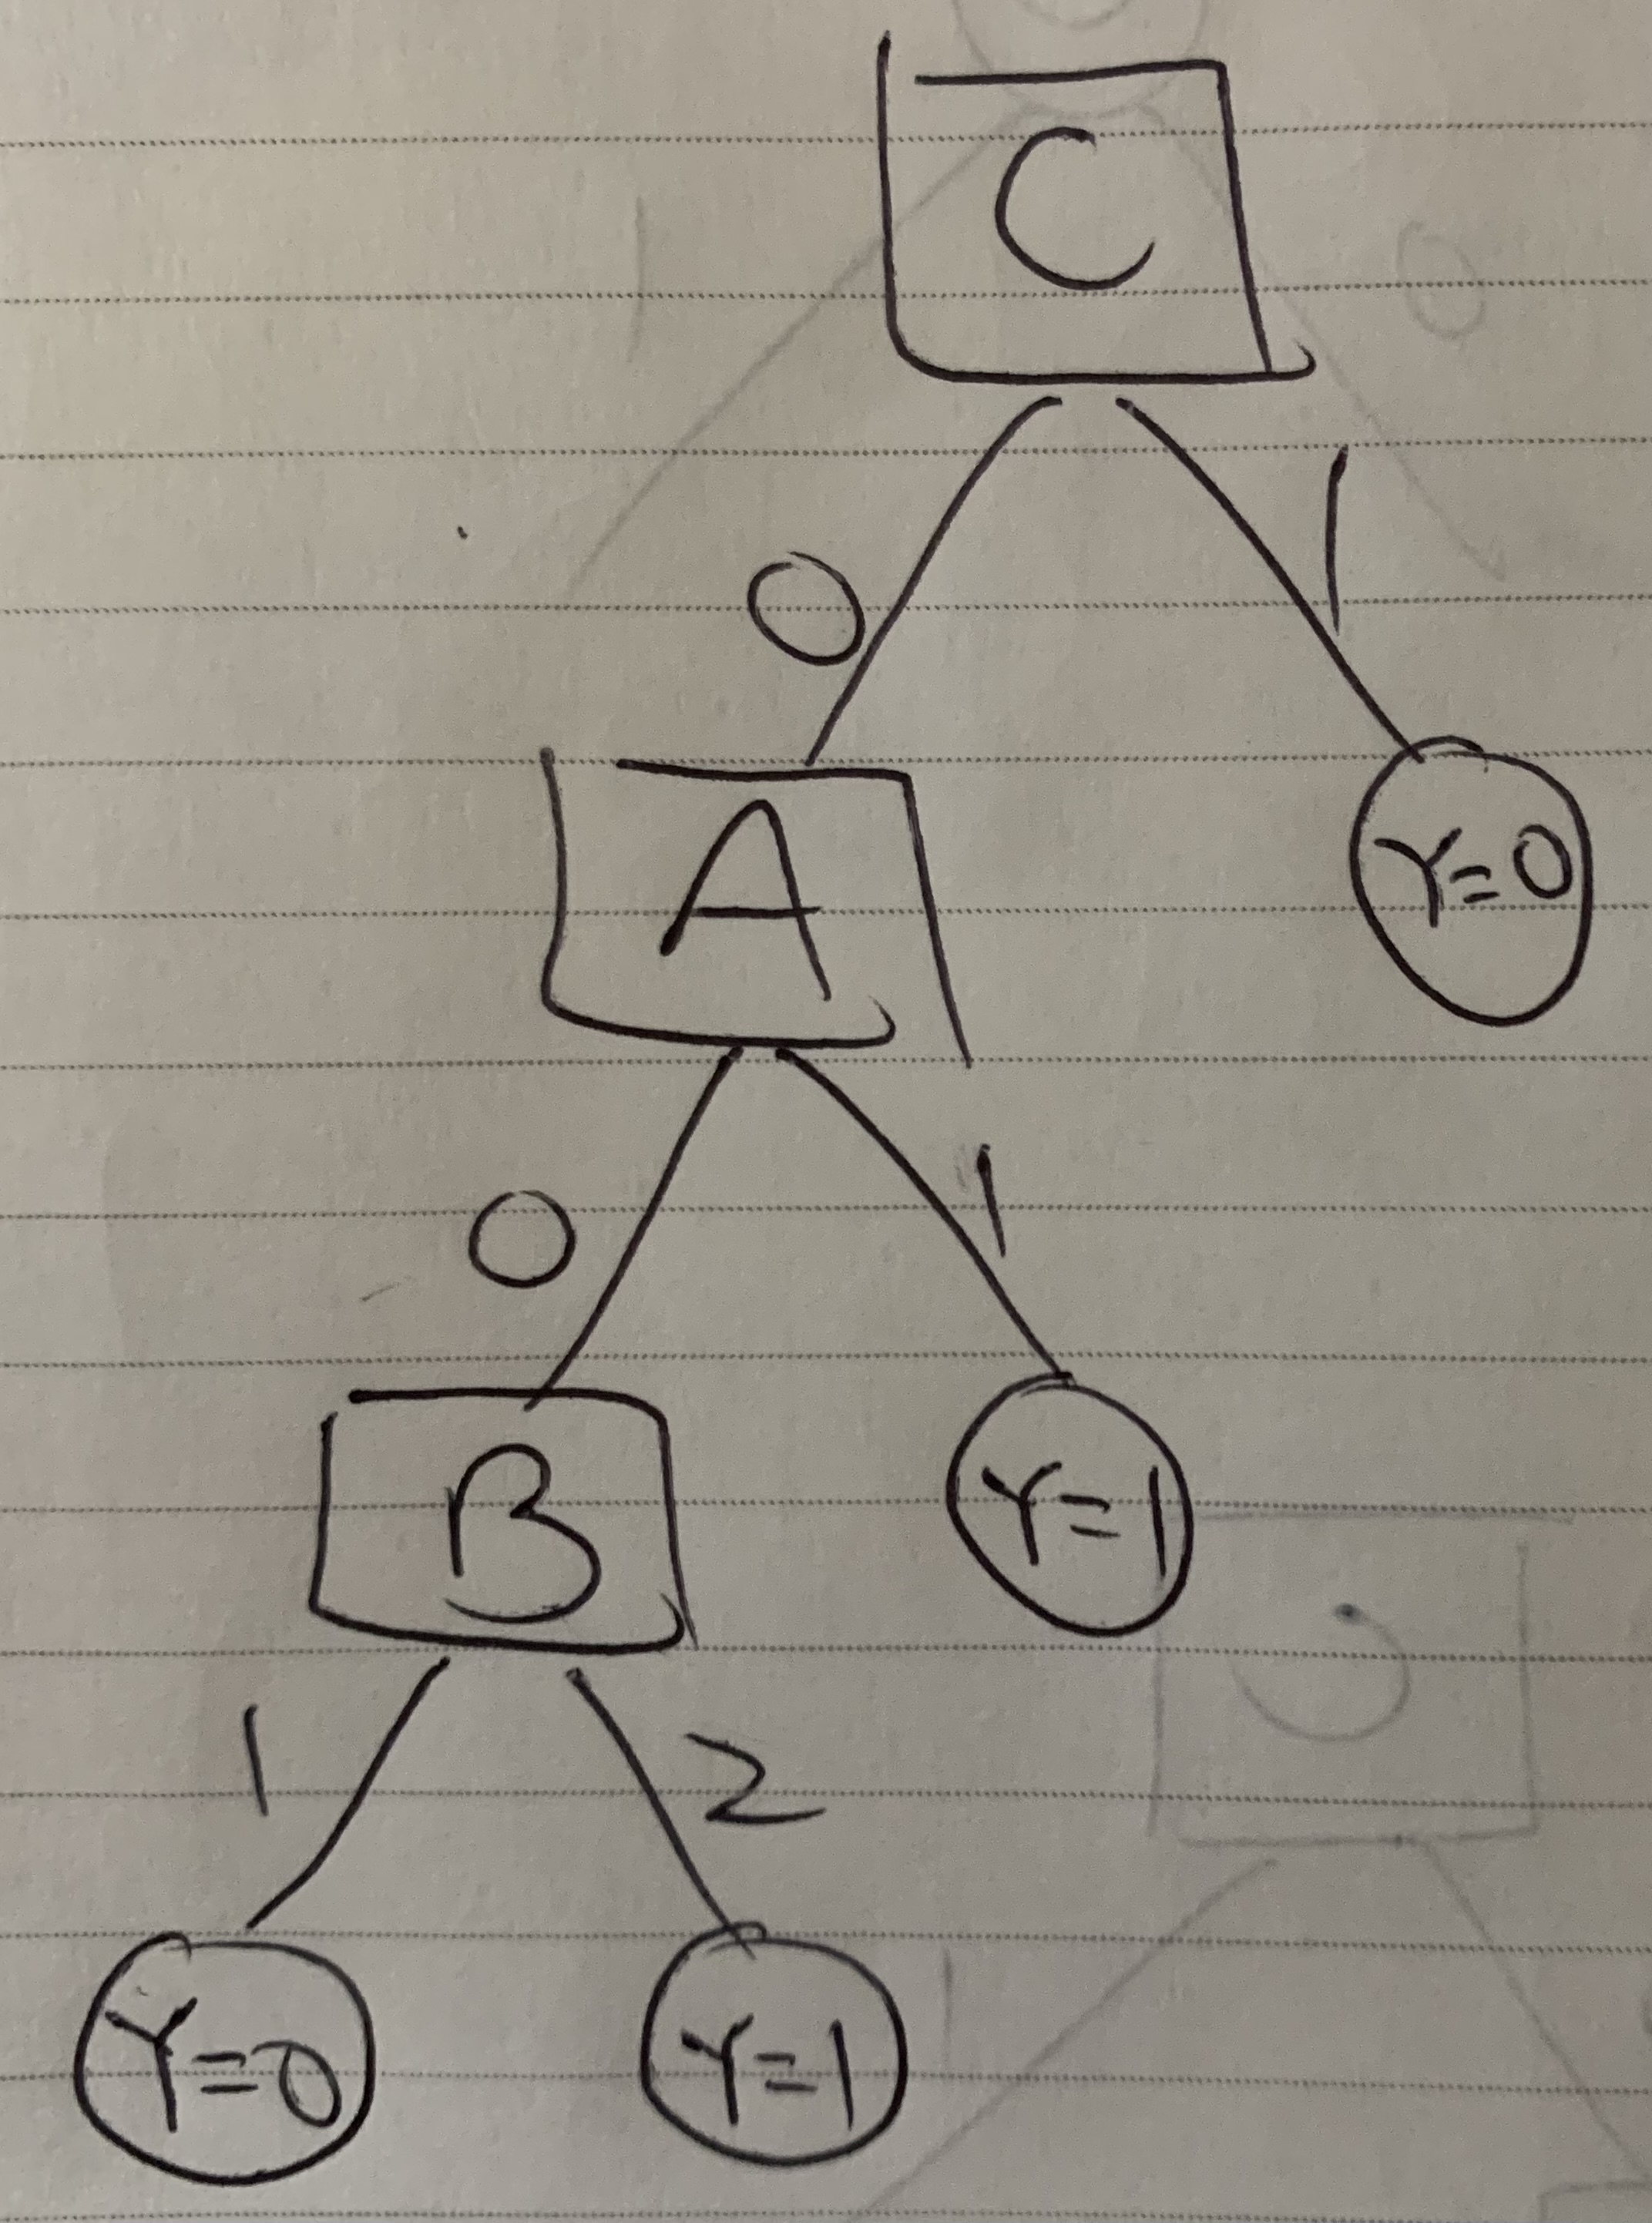
\includegraphics[width=0.5\linewidth]{DecTree.png}
    % % Change the "0.5\linewidth" part as necessary to make the picture fit in the box.
    \end{center}


    \end{your_solution}
    
\end{parts}\clearpage
\newpage
\sectionquestion{Pseudocode}
\label{sec:pseudo}

\begin{parts}
    
    \part In the programming assignment, you will need to implement three main tasks: training a decision tree on an arbitrary training set, predicting new values with a trained tree given an arbitrary input dataset, and evaluating your predictions against an arbitrary dataset's true labels. For this problem, we will focus on thinking through the algorithm for the \emph{second} task.
    
    Below, you will write pseudocode for the function \texttt{predict(node, example)}, which predicts the label of an \texttt{example} given a \texttt{node} of type \texttt{Node} representing the root of a \emph{trained} tree. You must approach this problem recursively and use the \texttt{Node} class we have given to you. 
    
    \begin{lstlisting}[escapechar=@]
class Node:
    def __init__(self, attr, v):
        self.attribute = attr
        self.left = None
        self.right = None
        self.vote = v
    
# (a) the left and right children of a node are denoted as
#     node.left and node.right respectively, each is of type Node
# (b) the attribute for a node is denoted as node.attribute and has
#     type str
# (c) if the node is a leaf, then node.vote of type str holds the 
#     prediction from the majority vote; if node is an internal
#     node, then node.vote has value None
# (d) assume all attributes have values 0 and 1 only; further
#     assume that the left child corresponds to an attribute value
#     of 1, and the right child to a value of 0

def predict(node, example):
    # example is a dictionary which holds the attributes and the
    # values of the attribute (ex. example['X'] = 0)
    
    if @\underline{$~~~$\textbf{Part (a)}$~~~$}@:
        return @\underline{$~~~$\textbf{Part (b)}$~~~$}@
    else:   
        @\underline{$~~~$\textbf{                   Part (c)          }$~~~$}@
        ________________
        ________________
        ________________
    

    \end{lstlisting}
    \begin{subparts}
    \subpart[2] Write the conditional statement of the base case of \texttt{predict(node, example)}. \\
    \begin{your_solution}[title=Your Answer,height=3.05cm]
        
    % INSERT YOUR ANSWER BELOW
    \begin{your_code_solution}
    	node.vote is not None
    \end{your_code_solution}
        
        
    \end{your_solution}

    \subpart[1] Write the return statement of the base case of \texttt{predict(node, example)}. \\

    \begin{your_solution}[title=Your Answer,height=3.05cm]
        
    % INSERT YOUR ANSWER BELOW
    \begin{your_code_solution}
    	node.vote
    \end{your_code_solution}
        
        
    \end{your_solution}
    
    \subpart[3] Write the recursive step of \texttt{predict(node, example)}. Limit your answer to 10 lines.\\
    \textbf{NOTE:} This may be a multi line solution.  \\
    \begin{your_solution}[title=Your Answer,height=7.05cm]
        
    % INSERT YOUR ANSWER BELOW
    \begin{your_code_solution}
    	if example[node.attribute] == 0:
    		predict(node.right, example)
    	else:
    		predict(node.left, example)

    \end{your_code_solution}
        
    \end{your_solution}
    \end{subparts}
\end{parts}\clearpage
\newpage
\sectionquestion{Empirical Questions}
\label{sec:empQ}

The following questions should be completed as you work through the programming portion of this assignment.

 \begin{parts}
    
    \part[4] Train and test your decision tree on the heart dataset and the education dataset with four different values of max-depth, $\{0,1,2,4\}$. Report your findings in the HW2 solutions template provided. A Decision Tree with max-depth 0 is simply a \emph{majority vote classifier}; a Decision Tree with max-depth 1 is called a \emph{decision stump}. (Please round each number to the fourth decimal place, e.g. 0.1234)
    
    \begin{center}
    \begin{tabular}{cc|c|c}
        % YOUR ANSWER
        \toprule
        {\bf Dataset}   & {\bf Max-Depth} & {\bf Train Error} & {\bf Test Error} \\
        \midrule
        heart & 0 & 0.49  & 0.4021  \\
        heart & 1 & 0.215  & 0.2784  \\
        heart & 2 & 0.215  & 0.3299  \\
        heart & 4 & 0.125  & 0.2577  \\
        \midrule
        education & 0 & 0.325  & 0.31  \\
        education & 1 & 0.195  & 0.23  \\
        education & 2 & 0.195  & 0.23  \\
        education & 4 & 0.13  & 0.16  \\
        \bottomrule
    \end{tabular}
    \end{center}
    
    
    \clearpage
    
    
    \part[3] For the heart disease (\texttt{heart}) dataset, create a \emph{computer-generated} plot showing error on the y-axis against depth of the tree on the x-axis. On a single plot, include \emph{both} training error and testing error, clearly labeling which is which.  That is, for each possible value of max-depth ($0, 1, 2, \ldots,$ m), where m $= $ number of attributes in the dataset, you should train a decision tree and report train/test error of the model's predictions. You should include an image file below using the provided, commented out code in \LaTeX{}, switching out \texttt{heart.png} to your file name as needed.
    
        \begin{your_solution}[title=Plot,height=15cm]
        % YOUR ANSWER 
         \begin{center}
         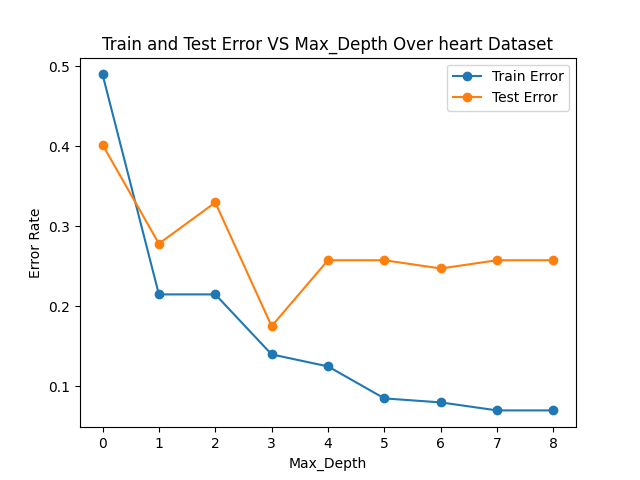
\includegraphics[width=0.9\linewidth]{heart.png}
         % Change the "0.5\linewidth" part as necessary to make the picture fit in the box.
         \end{center}
    \end{your_solution}


    \clearpage
    
    \part[2] \sone Suppose your research advisor asks you to run some model selection experiments and then report your results. You select the Decision Tree model's max-depth to be the one with lowest test error in metrics.txt and then report that model's test error as the performance of our classifier on held out test data. Is this a good experimental setup?
    

    \begin{checkboxes}
        % YOUR ANSWER
        \choice Yes, because we are using the test set in order to choose the best model.
        \choice No, because we should be using the \emph{training} set to optimize the max-depth, not the test set.
        \choice Yes, because we are not using the training set to tune hyperparameters.
        \CorrectChoice No, because we should be using a \emph{validation} set to optimize the max-depth, not the test set.
    \end{checkboxes}


    
    \part[2] \sone In this assignment, we used max-depth as our stopping criterion, and as a mechanism to prevent overfitting. Alternatively, we could stop splitting a node whenever the mutual information for the best attribute is lower than a threshold value. This threshold would be another hyperparameter. Theoretically, how would increasing this threshold value affect the number of nodes and depth of the learned trees?
    
    \begin{checkboxes}
        % YOUR ANSWER
        \CorrectChoice The higher this threshold value is, the \emph{smaller} depth and the \emph{fewer} nodes the decision tree contains.
        \choice The higher this threshold value is, the \emph{smaller} depth and the \emph{more} nodes the decision tree contains.
        \choice The higher this threshold value is, the \emph{higher} depth and the \emph{fewer} nodes the decision tree contains.
        \choice The higher this threshold value is, the \emph{higher} depth and the \emph{more} nodes the decision tree contains.
        \choice The depth and number of nodes in the decision tree will not vary as the threshold value increases.
    \end{checkboxes}

%     \clearpage
    
%     % \clearpage
    
%     \part[2] Print (do not handwrite!) the decision tree which is produced by your algorithm for the heart dataset with max depth 3. Instructions on how to print the tree could be found in section \ref{sec:printtree}.
    
%     \newsavebox{\outputbox}
%     \setbox\outputbox=\hbox{\begin{lstlisting}[backgroundcolor=\transparent{0}\color{white}]
% % YOUR ANSWER 
% % Text here will be compiled verbatim.
% % So do not add unnecessary indents

%     \end{lstlisting}}
    
%     \begin{your_solution}[title=Output,height=12cm]
%     \hspace{-1cm}
%     \usebox\outputbox
    

    
%     \end{your_solution}
    

    \clearpage
    
\end{parts}\clearpage
\newpage
\newpage
\section{Collaboration Questions}
After you have completed all other components of this assignment, report your answers to these questions regarding the collaboration policy. Details of the policy can be found \href{http://www.cs.cmu.edu/~mgormley/courses/10601/syllabus.html}{here}.
\begin{enumerate}
    \item Did you receive any help whatsoever from anyone in solving this assignment? If so, include full details.
    \item Did you give any help whatsoever to anyone in solving this assignment? If so, include full details.
    \item Did you find or come across code that implements any part of this assignment? If so, include full details.
\end{enumerate}

\begin{your_solution}[height=6cm]
% YOUR ANSWER 
\begin{enumerate}
	\item No.
	\item No.
	\item Yes, I find the following website (a) to know how to use typing to indicate the dimension of input and output array in a function, website (b) to figure out how to use regular expression to read error values in metrics files, and website (c) to know how plot multiple lines in a figure.
	\small
	\begin{enumerate}
		\item \url{https://stackoverflow.com/questions/75495212/type-hinting-numpy-arrays-and-batches}
		\item \url{https://docs.python.org/3/library/re.html#re.findall}
		\item \url{https://stackoverflow.com/questions/67392824/plot-two-lines-in-one-graph-with-each-line-own-y-values}
	\end{enumerate}
\end{enumerate}
\end{your_solution}
\newpage
\end{questions}

\section{Programming (72 points)}

Your goal in this assignment is to implement a binary classifier, entirely from scratch--specifically a Decision Tree learner. In addition, we will ask you to run some end-to-end experiments on two tasks (predicting whether or not a patient has heart disease / predicting the final grade for high school students) and report your results.
%
You will write two programs: \texttt{inspection.py} (Section \ref{sec:inspect}) and \texttt{decision\_tree.py} (Section \ref{sec:decisiontree}). The programs you write will be automatically graded using Gradescope.

\subsection{The Tasks and Datasets}
\label{sec:data}

\paragraph{Materials} Download the zip file from the course website. The zip file will have a handout folder that contains all the data that you will need in order to complete this assignment.

\paragraph{Starter Code} The handout will contain a preexisting \texttt{decision\_tree.py} file that itself contains some starter code for the assignment. While we do not require that you use the starter code in your final submission, we \emph{heavily} recommend building upon the structure laid out in the starter code.

\paragraph{Datasets}

The handout contains three datasets. Each one contains attributes and labels and is already split into training and testing data. The first line of each \lstinline{.tsv} file contains the name of each attribute, and \emph{the class label is always the last column}.

\begin{enumerate}
\item \textbf{heart:}
    The first task is to predict whether a patient has been (or will be) diagnosed with heart disease, based on available patient information. The attributes (aka. features) are: 
    \begin{enumerate}
        \item \lstinline{sex}: The sex of the patient---1 if the patient is male, and 0 if the patient is female.
        \item \lstinline{chest_pain}: 1 if the patient has chest pain, and 0 otherwise.
        \item \lstinline{high_blood_sugar}: 1 if the patient has high blood sugar ($>$120 mg/dl fasting), or 0 otherwise.
        \item \lstinline{abnormal_ecg}: 1 if exercise induced angina in the patient, and 0 otherwise. Angina is a type of severe chest pain.
        \item \lstinline{flat_ST}: 1 if the patient's ST segment (a section of an ECG) was flat during exercise, or 0 if it had some slope.
        \item \lstinline{fluoroscopy}: 1 if a physician used fluoroscopy, and 0 otherwise. Fluoroscopy is an imaging technique used to see the flow of blood through the heart.
        \item \lstinline{thalassemia}: 1 if the patient is known to have thalassemia, and 0 otherwise. Thalassemia is a blood disorder that may impair the oxygen-carrying capacity of the patient's red blood cells.
        \item \lstinline{heart_disease}: 1 if the patient was diagnosed with heart disease, and 0 otherwise. This is the class label you should predict.
    \end{enumerate}
    The training data is in \lstinline{heart_train.tsv}, and the test data in \lstinline{heart_test.tsv}.
\item \textbf{education:}
    The second task is to predict the final grade for high school students. The attributes (covariates, predictors) are student grades on 5 multiple choice assignments \emph{M1} through \emph{M5}, 4 programming assignments \emph{P1} through \emph{P4}, and the final exam \emph{F}. Values of 1 indicate that a student received an A, and 0 indicates that the student did not receive an A. The training data is in \newline \lstinline{education_train.tsv}, and the test data in \lstinline{education_test.tsv}.
\item \textbf{small:}
    We also include \lstinline{small_train.tsv} and \lstinline{small_test.tsv}---a small, purely for demonstration version of the \textbf{heart} dataset, with \emph{only} attributes \lstinline{chest_pain} and \lstinline{thalassemia}.  
    For this small dataset, the handout folder also contains the predictions from a reference implementation of a Decision Tree with max-depth 3 (see \lstinline{small_3_train.labels}, \lstinline{small_3_test.labels}, \lstinline{small_3_metrics.txt}).
    You can check your own output against these to see if your implementation is correct.
\end{enumerate}

\begin{notebox} \textbf{Note:}
For simplicity, all attributes are discretized into just two categories (i.e. each node will have at most two descendents). This applies to all the datasets in the handout, as well as the additional datasets on which we will evaluate your Decision Tree.
\end{notebox}

% \newpage
\subsection{Program \#1: Inspecting the Data (5 points)}
\label{sec:inspect}

    Create and write a program \texttt{inspection.py} to calculate the label entropy at the root (i.e. the entropy of the labels before any splits) and the error rate (the percent of incorrectly classified instances) of classifying using a majority vote (picking the label with the most examples). You do not need to look at the values of any of the attributes to do these calculations; knowing the labels of each example is sufficient. \textbf{Entropy should be calculated in bits using log base 2.}

\paragraph{Command Line Arguments}
The autograder runs and evaluates the output from the files  generated, using the following command:

\begin{tabular}{ll}
\begin{lstlisting}[language=Shell]
$ python inspection.py <input> <output>
\end{lstlisting}
\end{tabular}

Your program should accept two command line arguments: an input file and an output file. It should read the \lstinline{.tsv} input file (of the format described in Section \ref{sec:data}), compute the quantities above, and write them to the output file so that it contains:
\begin{quote}
\begin{verbatim}
entropy: <entropy value>
error: <error value>
\end{verbatim}
\end{quote}

\paragraph{Example}

For example, suppose you wanted to inspect the file \lstinline{small_train.tsv} and write out the results to \lstinline{small_inspect.txt}. You would run the following command:
%
\begin{lstlisting}[language=Shell]
$ python inspection.py small_train.tsv small_inspect.txt
\end{lstlisting}
%
Afterwards, your output file \lstinline{small_inspect.txt} should contain the following:
%
\begin{quote}
\begin{verbatim}
entropy: 1.000000
error: 0.500000
\end{verbatim}
\end{quote}
%
Our autograder will run your program on several input datasets to check that it correctly computes entropy and error, and will take minor differences due to rounding into account. You do not need to round your reported numbers! The autograder will automatically incorporate the right tolerance for float comparisons.

\begin{notebox}
For your own records, run your program on each of the datasets provided in the handout---this error rate for a \emph{majority vote} classifier is a baseline over which we would (ideally) like to improve.
\end{notebox}

% \newpage
\subsection{Program \#2: Decision Tree Learner (67 points)}
\label{sec:decisiontree}

In \texttt{decision\_tree.py}, implement a Decision Tree learner. This file should learn a decision tree with a specified maximum depth, print the decision tree in a specified format, predict the labels of the training and testing examples, and calculate training and testing errors.

\clearpage
\textbf{Your implementation must satisfy the following requirements:}
\begin{itemize}
\item Use mutual information to determine which attribute to split on.
\item Be sure you’re correctly weighting your calculation of mutual information. For a split on attribute X, $I(Y;X) = H(Y)-H(Y|X) = H(Y) - P(X=0)H(Y|X = 0) - P(X = 1)H(Y|X = 1)$.
\item As a stopping rule, only split on an attribute if the mutual information is $>$ 0. 
\item Do not grow the tree beyond a max-depth specified on the command line. For example, for a maximum depth of 3, split a node only if the mutual information is $>$ 0 and the current level of the node is $< 3$.
\item Use a majority vote of the labels at each leaf to make classification decisions. If the vote is tied, choose the label that is higher (i.e. $1$ should be chosen before $0$)
\item It is possible for different columns to have equal values for mutual information. In this case, you should split on the \emph{\textbf{first column to break ties}} (e.g. if column 0 and column 4 have the same mutual information, use column 0).
\item Do not hard-code any aspects of the datasets into your code. We may autograde your programs on hidden datasets that include different attributes and output labels.
\end{itemize}

\subsubsection{Getting Started}

Careful planning will help you to correctly and concisely implement your Decision Tree learner. Here are a few \emph{hints} to get you started:
\begin{itemize}
    \item Write helper functions to calculate entropy and mutual information.
    \item It is best to think of a Decision Tree as a collection of nodes, where nodes are either leaf nodes (where final decisions are made) or interior nodes (where we split on attributes). It is helpful to design a function to train a single node (i.e. a depth-0 tree), and then recursively call that function to create sub-trees.
    \item In the recursion, keep track of the depth of the current tree so you can stop growing the tree beyond the max-depth.
    \item Implement a function that takes a learned decision tree and data as inputs, and generates predicted labels. You can write a separate function to calculate the error of the predicted labels with respect to the given (ground-truth) labels.
    \item Be sure to correctly handle the case where the specified maximum depth is greater than the total number of attributes.
    \item Be sure to handle the case where max-depth is zero (i.e. a majority vote classifier). 
    \item Look under the FAQ post on Piazza for more useful clarifications about the assignment.
\end{itemize}

\begin{notebox}
Look out for the HW2 debugging checklist on Piazza!
\end{notebox}
\clearpage
\subsubsection{Command Line Arguments}

The autograder runs and evaluates the output from the files  generated, using the following command:

\begin{tabular}{ll}
\begin{lstlisting}[language=Shell]
$ python decision_tree.py [args...]
\end{lstlisting}
\end{tabular}

Where above \lstinline{[args...]} is a placeholder for seven command-line arguments: 
\texttt{<train input> <test input> <max depth> <train out> <test out> <metrics out> <print out>}. These arguments are described in detail below:
\begin{enumerate}
\item \lstinline{<train input>}: path to the training input \lstinline{.tsv} file (see Section \ref{sec:data})
\item \lstinline{<test input>}: path to the test input \lstinline{.tsv} file (see Section \ref{sec:data})
\item \lstinline{<max depth>}: maximum depth to which the tree should be built
\item \lstinline{<train out>}: path of output \lstinline{.txt} file to which the predictions on the \textit{training} data should be written (see Section \ref{sec:labels})
\item \lstinline{<test out>}: path of output \lstinline{.txt} file to which the predictions on the \emph{test} data should be written (see Section \ref{sec:labels})
\item \lstinline{<metrics out>}: path of the output \lstinline{.txt} file to which metrics such as train and test error should be written (see Section \ref{sec:metrics})
\item \lstinline{<print out>}: path of the output \lstinline{.txt} file to which the printed tree should be written (see Section \ref{sec:printtree})
\end{enumerate}

As an example, the following command line would run your program on the heart dataset and learn a tree with a max-depth of 2. The train predictions would be written to \lstinline{heart_2_train.txt}, the test predictions to \lstinline{heart_2_test.txt}, the metrics to \lstinline{heart_2_metrics.txt}, and the printed tree to \lstinline{heart_2_print.txt}.
%
\begin{lstlisting}[language=Shell]
$ python decision_tree.py heart_train.tsv heart_test.tsv 2 \ 
        heart_2_train.txt heart_2_test.txt heart_2_metrics.txt 
        \ heart_2_print.txt
\end{lstlisting}
%
The following example would run the same learning setup except with a max-depth of 3, and conveniently writing to analogously named output files, so you can can compare the two runs.
%
\begin{lstlisting}[language=Shell]
$ python decision_tree.py heart_train.tsv heart_test.tsv 3 \ 
        heart_3_train.txt heart_3_test.txt heart_3_metrics.txt 
        \ heart_3_print.txt
\end{lstlisting}

\subsubsection{Output: Labels Files}
\label{sec:labels}

Your program should write two output \lstinline{.txt} files containing the predictions of your model on training data (\lstinline{<train out>}) and test data (\lstinline{<test out>}). Each should contain the predicted labels for each example printed on a new line. Use `\texttt{\textbackslash n}' to create a new line.

Your labels should exactly match those of a reference decision tree implementation---this will be checked by the autograder by running your program and evaluating your output file against the reference solution.

% All labels are binary now -- this is implicit
% \textbf{Note}: You should output your predicted labels using the same string identifiers as the original training data: e.g., for the politicians dataset you should output democrat/republican and for the education dataset you should output A/notA.
%
The first few lines of an example output file is given below for the small dataset:
\begin{quote}
\begin{verbatim}
1
0
1
1
0
0
...
\end{verbatim}
\end{quote}

\subsubsection{Output: Metrics File}
\label{sec:metrics}

Generate another file where you should report the training error and testing error. This file should be written to the path specified by the command line argument \lstinline{<metrics out>}. Your reported numbers should be within 0.0001 of the reference solution. You do not need to round your reported numbers! The autograder will automatically incorporate the right tolerance for float comparisons. The file should be formatted as follows:

\begin{quote}
\begin{verbatim}
error(train): 0.214286
error(test): 0.285714
\end{verbatim}
\end{quote}

The values above correspond to the results from training a tree of depth 3 on \texttt{small\_train.tsv} and testing on \texttt{small\_test.tsv}. (Note that there is one space between the colon and value.)


\subsubsection{Output: Printing the Tree}
\label{sec:printtree}

You must write a function to pretty-print your learned decision tree. (This will also help you debug!) Generate another file where you report the printed tree. This file should be written to the path specified by the command line argument \lstinline{<print out>}. \textbf{Your function should print your tree only \emph{after} you are done generating the fully-trained tree.} Each row should correspond to a node in the tree. \textbf{The branch that corresponds to 0 should be printed before the branch that corresponds to 1.} 

A simple breakdown of each row within the pretty-print tree is as follows: 
\begin{enumerate}
    \item $d$ copies of the string `\texttt{|}' corresponding to the depth $d$ of the current node 
    \item \texttt{<Feature most recently split on (if any)> = <0 or 1>:}
    \item \texttt{[<\#0s> 0/<\#1s> 1]} (sufficient statistics of data at current node)
\end{enumerate}

Here is a reference output for printing the decision tree. 
\begin{lstlisting}[language=Shell]
$ python decision_tree.py small_train.tsv small_test.tsv 2 \ 
small_2_train.txt small_2_test.txt small_2_metrics.txt 
\ small_2_print.txt

[14 0/14 1]
| chest_pain = 0: [4 0/12 1]
| | thalassemia = 0: [3 0/4 1]
| | thalassemia = 1: [1 0/8 1]
| chest_pain = 1: [10 0/2 1]
| | thalassemia = 0: [7 0/0 1]
| | thalassemia = 1: [3 0/2 1]
\end{lstlisting}

\textbf{Note: }Your format do not need to match this output exactly to receive full points as we give flexibility with spacing. However, \textbf{each node of the tree must be printed in a separate line}.
Some examples of valid printing format include:
\begin{lstlisting}[language=Shell]
||thalassemia=0:[3 0/4 1]
||thalassemia=0:[3 0 / 4 1]
|  |  thalassemia = 0:[ 3 0/4 1 ]
...
\end{lstlisting}


You should also be careful that the tree might not be full. For example, with a different subset of the small dataset, there may be no nodes under \lstinline{chest_pain = 0} if all labels are the same.\\

% \clearpage
The following pretty-print shows the education dataset with max-depth 3.  Use this example to check your code before submitting to the autograder.  

\begin{lstlisting}[language=Shell]
$ python decision_tree.py education_train.tsv education_test.tsv 3 \
edu_3_train.txt edu_3_test.txt edu_3_metrics.txt edu_3_print.txt

[65 0/135 1]
| F = 0: [42 0/16 1]
| | M2 = 0: [27 0/3 1]
| | | M4 = 0: [22 0/0 1]
| | | M4 = 1: [5 0/3 1]
| | M2 = 1: [15 0/13 1]
| | | M4 = 0: [14 0/7 1]
| | | M4 = 1: [1 0/6 1]
| F = 1: [23 0/119 1]
| | M4 = 0: [21 0/63 1]
| | | M2 = 0: [18 0/26 1]
| | | M2 = 1: [3 0/37 1]
| | M4 = 1: [2 0/56 1]
| | | P1 = 0: [2 0/15 1]
| | | P1 = 1: [0 0/41 1]
\end{lstlisting}

The numbers in brackets give the number of positive and negative labels from the training data in that part of the tree. For the example above, the first line indicates that there at 65 zero-labels and 135 one-labels in the entire tree, and the second line indcates that there are 42 zero-labels and 16 one-labels in the branch where F = 0.

\begin{notebox}
At this point, you should be able to go back and answer questions 1-4 in the ``Empirical Questions" section of this handout.  Write your solutions in the template provided. \end{notebox}

\begin{comment}
    \subsection{Evaluation}
    In addition to the politician and education datasets, our autograder will test your code on two more datasets, which will not be shown to you. One set contains information about various cars, and whether or not consumers decided to buy them. The other contains data about songs, and whether or not they became top hits. The data will be in .tsv files formatted like the ones provided, again with the class as the last column. Shown below are the attributes and the values they can take: 
    
    Music data:
    
    \begin{itemize}
    \item \texttt{Attribute:year('before1950'or'after1950')}
    \item \texttt{Attribute:solo('yes'or'no')}
    \item \texttt{Attribute:vocal('yes'or'no')}
    \item \texttt{Attribute:length('morethan3min'or'lessthan3min')}
    \item \texttt{Attribute:original('yes'or'no')}
    \item \texttt{Attribute:tempo('fast'or'slow')}
    \item \texttt{Attribute:folk('yes'or'no')}
    \item \texttt{Attribute:classical('yes'or'no')}
    \item \texttt{Attribute:rhythm('yes'or'no')}
    \item \texttt{Attribute:jazz('yes'or'no')}
    \item \texttt{Attribute:rock('yes'or'no')}
    \item \texttt{Class Label:hit('yes'or'no')}
    \end{itemize}
    
    Cars data:
    
    \begin{itemize}
    \item \texttt{Attribute:buying('expensive'or'cheap')}
    \item \texttt{Attribute:maint('high'or'low')}
    \item \texttt{Attribute:doors('Two'or'MoreThanTwo')}
    \item \texttt{Attribute:length('morethan3min'or'lessthan3min')}
    \item \texttt{Attribute:person('Two'or'MoreThanTwo')}
    \item \texttt{Attribute:boot('large'or'small')}
    \item \texttt{Attribute:safety('high'or'low')}
    \item \texttt{Class Label:class('yes'or'no')}
    \end{itemize}
    
    Please ensure your solution can handle data with these values.
 
\end{comment}
    
\subsection{Submission Instructions}

\paragraph{Programming}
Please ensure you have completed the following files for submission.


\begin{verbatim}
inspection.py
decision_tree.py
\end{verbatim}

When submitting your solution, make sure to select and upload both files. \textbf{Any other files will be deleted.} Ensure the files have the exact same spelling and letter casing as above. You can either directly zip the two files (by selecting the two files and compressing them -- do not compress the folder containing the files) or directly drag them to Gradescope for submission. \textbf{Do NOT submit a Python notebook file (*.ipynb; Jupyter notebook or Google Colab notebook file).}


\paragraph{Written Questions}
Make sure you have completed all questions from Written component (including the collaboration policy questions) in the template provided.  When you have done so, please submit your document in \textbf{PDF format} to the corresponding assignment slot on Gradescope.



\newpage

\end{document}